\documentclass[landscape,paperwidth=72in,paperheight=36in,fontscale=0.2,margin=2.5cm]{baposter} % Adjust the font scale/size here

\usepackage{graphicx} % Required for including images
\graphicspath{{figures/}} % Directory in which figures are stored

\usepackage{amssymb,amsmath,amsthm}
\usepackage{enumitem} % Used to reduce itemize/enumerate spacing

\newcommand{\compresslist}{ % Define a command to reduce spacing within itemize/enumerate environments, this is used right after \begin{itemize} or \begin{enumerate}
    \setlength\itemsep{-0.2em}
}
\renewcommand{\labelitemi}{$\blacktriangleright$}
\setlist[itemize]{leftmargin=*}
\definecolor{UCFGold}{HTML}{FFCC00} % Defines the color used for content box headers


\newcommand{\KL}{\mathbb{KL}}
\newcommand{\B}{\mathbf}
\newcommand{\Bs}{\boldsymbol}
\DeclareMathOperator*{\argmax}{arg\,max}
\DeclareMathOperator*{\argmin}{arg\,min}

\theoremstyle{plain}
\newtheorem{theorem}{Theorem}[section]
\renewcommand{\thetheorem}{\arabic{theorem}} % Redefine counter representation


\begin{document}

\begin{poster}
{
columns=12,
textborder=none, % Format of the border around content boxes, can be: none, bars, coils, triangles, rectangle, rounded, roundedsmall, roundedright or faded
headerborder=none, % Adds a border around the header of content boxes
headershape=smallrounded, % Specify the rounded corner in the content box headers, can be: rectangle, small-rounded, roundedright, roundedleft or rounded
colspacing=1em, % Column spacing
bgColorOne=white, % Background color for the gradient on the left side of the poster
bgColorTwo=white, % Background color for the gradient on the right side of the poster
borderColor=UCFGold, % Border color
headerColorOne=UCFGold, % Background color for the header in the content boxes (left side)
headerColorTwo=UCFGold, % Background color for the header in the content boxes (right side)
headerFontColor=black, % Text color for the header text in the content boxes
boxColorOne=white, % Background color of the content boxes
eyecatcher=false, % Set to false for ignoring the left logo in the title and move the title left
headerheight=0.11\textheight, % Height of the header
headerfont=\large\bf, % Large, bold and sans serif font in the headers of content boxes
%textfont={\setlength{\parindent}{1.5em}}, % Uncomment for paragraph indentation
linewidth=1pt % Width of the border lines around content boxes
}

%%%%%%%%%%%%%%%%%%%%%%%%%%%%%%%%%%%%%%%%%%%%%%%%%%%%%%%%%%%%%%%%%%%%%%%%%%%%%%%%%%%%%%
{\vspace*{0.4em}\bf{\huge Unearthing InSights into Mars: Unsupervised Source Separation with Limited Data}\vspace{0.3em}}
{{Ali Siahkoohi, Rudy Morel, Maarten V. de Hoop, Erwan Allys, Grégory Sainton, and Taichi Kawamura}\vspace{0.4em}}
{{
\includegraphics[height=5.5em]{luqi-with-text.png}\hspace{1em}
\includegraphics[height=5.5em]{ucf-logo.png}}} % LuQi group logo and UCF logo

%%%%%%%%%%%%%%%%%%%%%%%%%%%%%%%%%%%%%%%%%%%%%%%%%%%%%%%%%%%%%%%%%%%%%%%%%%%%%%%%%%%%%%
\headerbox{Problem statement and contributions}{name=abstract,column=0,span=3,row=0}{

\textbf{Unsupervised source separation.} Retrieving unknown source signals recorded through a mixing operator, with limited prior knowledge about the sources, and only access to a dataset of signal mixtures.

\medskip

\textbf{Challenges:}
\vspace{-0.75em}
\begin{itemize}
    \compresslist
    \item inherent non-uniqueness
    \item lacking expert knowledge regarding sources
    \item limited access to training data ($\sim 50$ data snippets)
\end{itemize}

\vspace{-0.25em}
\textbf{Our contribution.} An unsupervised source separation method applicable to domains with limited access to data, e.g., when dealing with extraterrestrial data.

\vspace{-.75em}
}

%%%%%%%%%%%%%%%%%%%%%%%%%%%%%%%%%%%%%%%%%%%%%%%%%%%%%%%%%%%%%%%%%%%%%%%%%%%%%%%%%%%%%%
\headerbox{Example: Marsquake cleaning}{name=network,column=0,span=3,below=abstract}{

\begin{center}
    \centering
    
\includegraphics[width=1.0\linewidth]{marsquake/S1133c/real-data.png}
    
\includegraphics[width=1.0\linewidth]{marsquake/S1133c/marsquake.png}
    
\includegraphics[width=1.0\linewidth]{marsquake/S1133c/background.png}
\end{center}

\vspace{-1em}

{\small \textbf{Figure 1:} Unsupervised separation of background noise, including thermally induced microtilts (glitches), from a marsquake recorded during the NASA InSight mission.}
}

%%%%%%%%%%%%%%%%%%%%%%%%%%%%%%%%%%%%%%%%%%%%%%%%%%%%%%%%%%%%%%%%%%%%%%%%%%%%%%%%%%%%%%
\headerbox{Wavelet Scattering Covariances}{name=cov,column=3,row=0,span=4}{

A quasi-block diagonal approximation to second-order moments of wavelet scattering network output $\Phi(\B{x}) := \mathbb{E}\,\big[S(\B{x}) \,S(\B{x})^\top\big]$
%
\begin{itemize}
    \compresslist
    \item $S(\B{x}) := \begin{bmatrix}
                \B{W}\B{x},
                \B{W}|\B{W}\B{x}|
                \end{bmatrix}^{\top}$ and $\B{W}$ the wavelet transform
    \item expectation over time (estimated by average pooling)
    \item a low-dimensional representation of stochastic processes
    \item capable of capturing non-Gaussian properties
    % \item domain knowledge (signal process) rich inductive bias
    \item scalable as block matrices in $S(\B{x})\, S(\B{x})^\top$ are quasi-diagonal
\end{itemize}

\vspace{-1.5em}

}


%%%%%%%%%%%%%%%%%%%%%%%%%%%%%%%%%%%%%%%%%%%%%%%%%%%%%%%%%%%%%%%%%%%%%%%%%%%%%%%%%%%%%%
\headerbox{Unsupervised Source Separation}{name=uss,column=3,span=4,below=cov}{

\textbf{Objective.} Retrieve unknown source $\B{s}(t)$ from $\B{x}(t) = \B{s}(t) +\B{n}(t)$ using observed samples $\{\B{n}_k(t)\}_{k=1}^{K}$ as prior information.

\vspace{0.5em}

\textbf{Proposed method.} Cast source separation as an optimization problem in the wavelet scattering covariance representation space

\begin{equation*}
\begin{aligned}
\B{\widehat{s}} := \argmin_{\B{s}}\, \Big[
    \mathcal{L}_{\text{data}} (\B{s})
    + \mathcal{L}_{\text{prior}} (\B{s})
    + \mathcal{L}_{\text{cross}} (\B{s}) \Big]
\end{aligned}
\end{equation*}

\vspace{-1em}

\begin{align*}
    \text{data misfit loss:} \quad \mathcal{L}_{\text{data}} \left(\B{s}\right) & =
    \frac{1}{K}\sum_{k=1}^K
    \frac{\left\|\Phi\left(\B{s}
    + \B{n}_k\right)
    - \Phi\left(\B{x}\right)\right\|_2^2}
    {\sigma^2\left(\Phi\left(\B{x}+\B{n}_k\right)\right)}, \\
    \text{prior loss:} \quad \mathcal{L}_{\text{prior}} \left(\B{s}\right) & =
    \frac{1}{K}\sum_{k=1}^K
    \frac{ \left\|\Phi\left(\B{x}
    - \B{s}\right)
    - \Phi\left(\B{n}_k\right)\right\|_2^2}{\sigma^2\left(\Phi\left(\B{n}_k\right)\right)}, \\
    \text{cross-covariance loss:} \quad \mathcal{L}_{\text{cross}} (\B{s}) & =
    \frac{1}{K}\sum_{k=1}^K\frac{\left\|\Phi\left(\B{s}, \B{n}_k\right)\right\|_2^2}{\sigma^2\left(\Phi\left(\B{x},\B{n}_k\right)\right)}
\end{align*}

\vspace{-1em}

}

%%%%%%%%%%%%%%%%%%%%%%%%%%%%%%%%%%%%%%%%%%%%%%%%%%%%%%%%%%%%%%%%%%%%%%%%%%%%%%%%%%%%%%
\headerbox{Conclusion}{name=conclusion,column=3,span=4,above=bottom}{

We reaped the benefits of the inductive bias built into scattering covariances, enabling us to obtain low-dimensional representations that characterize a wide range of non-Gaussian properties of stochastic processes without pretraining, leading to a data frugal source separation method.
\vspace{0.2em}
}

%%%%%%%%%%%%%%%%%%%%%%%%%%%%%%%%%%%%%%%%%%%%%%%%%%%%%%%%%%%%%%%%%%%%%%%%%%%%%%%%%%%%%%
\headerbox{Probabilistic recovery guarantee}{name=theorem,row=0,column=7,span=5}{

\begin{theorem}
Let $\mathbf{x}= \B{s} + \B{n}$ with $\mathbf{s}$ and $\mathbf{n}$ two independent processes.
Let us assume we have two processes $\widehat{\mathbf{s}}$ and $\widehat{\mathbf{n}}$ with $\mathbf{x}= \widehat{\B{s}} + \widehat{\B{n}}$ such that:
\vspace*{-0.5em}
\begin{enumerate}[label=(\roman*)]
\label{main-theo}
    \compresslist
    \item \label{assump:maxH_n} $\mathbf{n}$ has a maximum entropy distribution under moment constraints $\mathbb{E}\{\Phi(\mathbf{n})\}$
    \item \label{assump:maxH_nt} $\widehat{\mathbf{n}}$ has a maximum entropy distribution under moment constraints $\mathbb{E}\{\Phi(\widehat{\mathbf{n}})\}$
    \item\label{assump:samestat} $\mathbb{E}\{\Phi(\widehat{\mathbf{n}})\}=\mathbb{E}\{\Phi(\mathbf{n})\}$
    \item\label{assump:indep} $\widehat{\mathbf{s}}$ and $\widehat{\mathbf{n}}$ are independent
    \item\label{assump:nonzeroFourier}
    The Fourier transform $\widehat{p}_\mathbf{n}$ of the distribution $p_\mathbf{n}$ of $\mathbf{n}$ is non-zero everywhere.
\end{enumerate}
\vspace*{-0.5em}
$\Rightarrow$ $\mathbf{n}\overset{d}{=}\widehat{\mathbf{n}}$ and $\mathbf{s}\overset{d}{=}\widehat{\mathbf{s}}$ where the equality is on the distribution of the processes.
\end{theorem}

\vspace{-1.5em}

}

%%%%%%%%%%%%%%%%%%%%%%%%%%%%%%%%%%%%%%%%%%%%%%%%%%%%%%%%%%%%%%%%%%%%%%%%%%%%%%%%%%%%%%
\headerbox{Stylized example: Turbulent signal separation}{name=multifractal,column=7,span=5,below=theorem}{

{\hspace*{-1.8em}
\begin{tabular}{cc}
  \begin{minipage}[b]{0.52\linewidth}
    \centering
    
\includegraphics[width=\linewidth]{turbulance_max_itr-500_window_size-2048_j-8-8_q-1-1_R-100_tol_optim-0.1_indep_loss_w-1.0_x_loss_w-1.0_process_name-mrw_type-turbulence_wavelet-battle_lemarie/x_true.png}
  \end{minipage} &
  \hspace{-1.5em}
  \begin{minipage}[b]{0.52\linewidth}
    \centering
    
\includegraphics[width=\linewidth]{turbulance_max_itr-500_window_size-2048_j-8-8_q-1-1_R-100_tol_optim-0.1_indep_loss_w-1.0_x_loss_w-1.0_process_name-mrw_type-turbulence_wavelet-battle_lemarie/x_obs.png}
  \end{minipage}
  \\
  \begin{minipage}[b]{0.52\linewidth}
    \centering
    
\includegraphics[width=\linewidth]{turbulance_max_itr-500_window_size-2048_j-8-8_q-1-1_R-100_tol_optim-0.1_indep_loss_w-1.0_x_loss_w-1.0_process_name-mrw_type-turbulence_wavelet-battle_lemarie/x_hat_with_reg.png}
  \end{minipage} &
  \hspace{-1.5em}
  \begin{minipage}[b]{0.52\linewidth}
    \centering
    
\includegraphics[width=\linewidth]{turbulance_max_itr-500_window_size-2048_j-8-8_q-1-1_R-100_tol_optim-0.1_indep_loss_w-1.0_x_loss_w-1.0_process_name-mrw_type-turbulence_wavelet-battle_lemarie/error.png}
  \end{minipage}
\end{tabular}
}
{\small \textbf{Figure 2:} Unsupervised source separation applied to the multifractal random walk data with a turbulent additive signal. The vertical
axis is the same for all the plots.}

\vspace{-1em}

}

%%%%%%%%%%%%%%%%%%%%%%%%%%%%%%%%%%%%%%%%%%%%%%%%%%%%%%%%%%%%%%%%%%%%%%%%%%%%%%%%%%%%%%
\headerbox{Separating glitches: Seismic data from Mars}{name=deglitching,column=7,span=5,below=multifractal}{

{\hspace*{-1.8em}
\begin{tabular}{cc}
  \begin{minipage}[b]{0.52\linewidth}
    \centering
    
\includegraphics[width=\linewidth]{deglitching_detrend_idx_max_itr-1000_window_size-2048_j-8-8_q-1-1_R-50_tol_optim-0.1_indep_loss_w-1.0_x_loss_w-1.0_type-raw_normalize-1_wavelet-battle_lemarie_glitch_idx-3/x_obs.png}
  \end{minipage} &
  \hspace{-1.5em}
  \begin{minipage}[b]{0.52\linewidth}
    \centering
    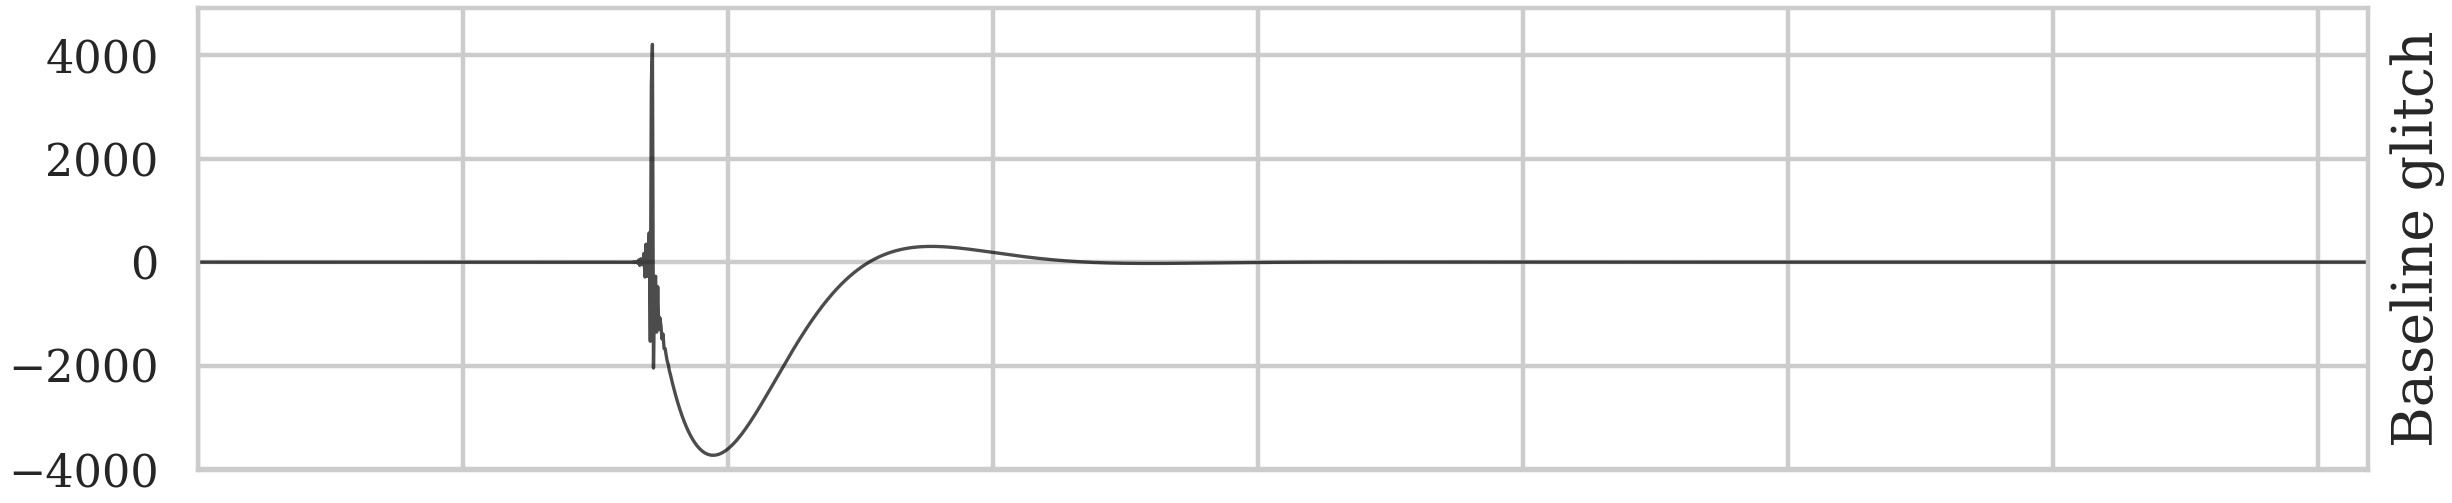
\includegraphics[width=\linewidth]{deglitching_detrend_idx_max_itr-1000_window_size-2048_j-8-8_q-1-1_R-50_tol_optim-0.1_indep_loss_w-1.0_x_loss_w-1.0_type-raw_normalize-1_wavelet-battle_lemarie_glitch_idx-3/g_base.png}
  \end{minipage}
  \\
  \begin{minipage}[b]{0.52\linewidth}
    \centering
    
\includegraphics[width=\linewidth]{deglitching_detrend_idx_max_itr-1000_window_size-2048_j-8-8_q-1-1_R-50_tol_optim-0.1_indep_loss_w-1.0_x_loss_w-1.0_type-raw_normalize-1_wavelet-battle_lemarie_glitch_idx-3/x_hat_with_reg.png}
  \end{minipage} &
  \hspace{-1.5em}
  \begin{minipage}[b]{0.52\linewidth}
    \centering
    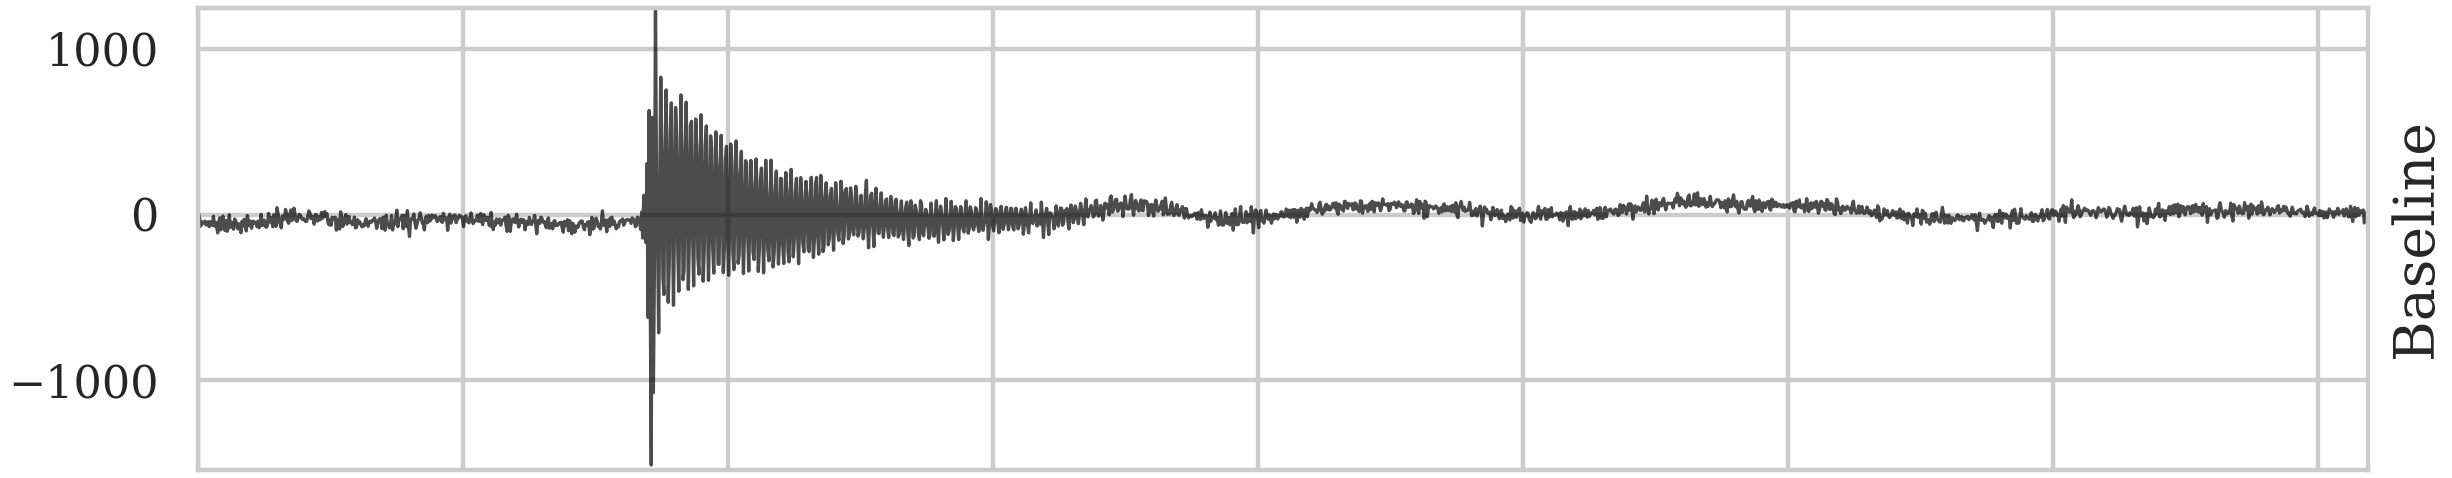
\includegraphics[width=\linewidth]{deglitching_detrend_idx_max_itr-1000_window_size-2048_j-8-8_q-1-1_R-50_tol_optim-0.1_indep_loss_w-1.0_x_loss_w-1.0_type-raw_normalize-1_wavelet-battle_lemarie_glitch_idx-3/x_base.png}
  \end{minipage}
\end{tabular}
}
{\small \textbf{Figure 3:} Unsupervised source separation for glitch removal. Our approach successfully separates the glitch using only glitch-free data snippets, while the baseline approach fails to accurately characterize the glitch, resulting in significant residual oscillations.}

}

\end{poster}
\end{document}